\documentclass{minimal}

% Tikz
\usepackage{pgf}
\usepackage{tikz}

\tikzset{
 	vertex/.style={draw=none,circle,fill=black,inner sep=2pt},
	edge/.style={draw,black,thick},
	thinedge/.style={draw,black,line width=.4pt},
	dedge/.style={draw,black,line width=.4pt,dashed}
}

\begin{document}

\begin{center}
 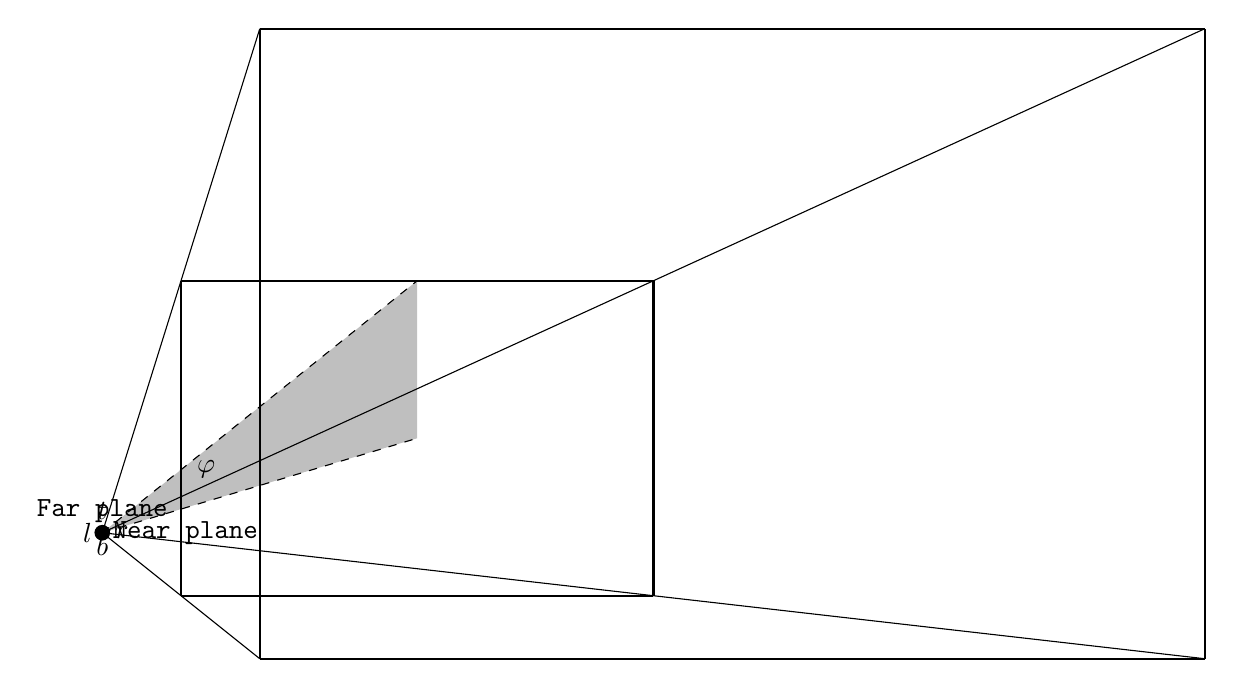
\begin{tikzpicture}[x  = {(1cm,0.0cm)},
                     y  = {(0.0cm,1.0cm)},
                     z  = {(2.0cm,0.6cm)}]
 
\coordinate (O) at (0,0,0);

\coordinate (lo) at (-3,2,2);
\coordinate (ro) at (3,2,2);
\coordinate (lu) at (-3,-2,2);
\coordinate (ru) at (3,-2,2);

\coordinate (LO) at (-6,4,4);
\coordinate (RO) at (6,4,4);
\coordinate (LU) at (-6,-4,4);
\coordinate (RU) at (6,-4,4);

\coordinate (c) at (0, 0, 2);
\coordinate (co) at (0, 2, 2);

\draw[fill=gray,draw=none,opacity=0.5] (O) -- (c) -- (co);
%\draw[fill=gray,opacity=0.5] (O) -- (17:1.2cm) arc (17:21.5:6cm);

\draw[edge] (lo) to (ro) node[pos=.5,above=.1em] {$t$};
\draw[edge] (lo) to (lu) node[pos=.5,left] {$l$};
\draw[edge] (ro) to (ru) node[pos=.5,right=.1em] {$r$} node[pos=.15,right] {$\texttt{Near plane}$};
\draw[edge] (lu) to (ru) node[pos=.5,above=.-1.2em] {$b$};

\draw[edge] (LO) to (RO) node[pos=.5,above] {$\texttt{Far plane}$} {};
\draw[edge] (LO) to (LU) {};
\draw[edge] (RO) to (RU) {};
\draw[edge] (LU) to (RU) {};

\draw[thinedge] (O) to (RO) {};
\draw[thinedge] (O) to (LO) {};
\draw[thinedge] (O) to (RU) {};
\draw[thinedge] (O) to (LU) {};

\draw[dedge] (O) to node[pos=.33,above=.5em]{$\varphi$} (c) {};
\draw[dedge] (O) to (co) {};

\node[vertex] at (O) {};

%\draw[->, thick] (-0.4,3) arc (0:320:20pt);

\end{tikzpicture}
\end{center}

\end{document}
